\documentclass[12pt,a4paper]{report}
\usepackage{fontspec}
\usepackage{xeCJK}
\usepackage{enumerate}
\usepackage{graphicx}
\usepackage{wallpaper}
\usepackage{tikz}
\usepackage{titlesec, titletoc} %设置标题格式
\usepackage[top=1 in,bottom=1 in,left=1.25 in,right=1.25 in]{geometry}
\usepackage{amsthm}
\setCJKmainfont{黑体}
\XeTeXlinebreaklocale zh
\XeTeXlinebreakskip = 0pt plus 1pt
\dottedcontents{chapter}[0.0em]{\vspace{0.5em}}{0.0em}{5pt}
\dottedcontents{section}[1.16cm]{}{1.8em}{5pt}
\dottedcontents{subsection}[2.00cm]{}{2.7em}{5pt}
\dottedcontents{subsubsection}[2.86cm]{}{3.4em}{5pt}
\setlength{\parindent}{2em} %段首缩进两格
\setlength{\baselineskip}{1.8em} %中文行距
\setlength{\parskip}{1ex} %段距
\newcommand{\chuhao}{\fontsize{42pt}{\baselineskip}\selectfont}
\newcommand{\xiaochu}{\fontsize{36pt}{\baselineskip}\selectfont}
\newcommand{\yihao}{\fontsize{26pt}{\baselineskip}\selectfont}
\newcommand{\xiaoyi}{\fontsize{24pt}{\baselineskip}\selectfont}
\newcommand{\erhao}{\fontsize{22pt}{\baselineskip}\selectfont}
\newcommand{\xiaoer}{\fontsize{18pt}{\baselineskip}\selectfont}
\newcommand{\sanhao}{\fontsize{16pt}{\baselineskip}\selectfont}
\newcommand{\xiaosan}{\fontsize{15pt}{\baselineskip}\selectfont}
\newcommand{\sihao}{\fontsize{14pt}{\baselineskip}\selectfont}
\newcommand{\banxiaosi}{\fontsize{13pt}{\baselineskip}\selectfont}
\newcommand{\xiaosi}{\fontsize{12pt}{\baselineskip}\selectfont}
\newcommand{\dawu}{\fontsize{11pt}{\baselineskip}\selectfont}
\newcommand{\wuhao}{\fontsize{10.5pt}{\baselineskip}\selectfont}
\newcommand{\xiaowu}{\fontsize{9pt}{\baselineskip}\selectfont}
\newcommand{\liuhao}{\fontsize{7.5pt}{\baselineskip}\selectfont}
\newcommand{\xiaoliu}{\fontsize{6.5pt}{\baselineskip}\selectfont}
\newcommand{\qihao}{\fontsize{5.5pt}{\baselineskip}\selectfont}
\newcommand{\bahao}{\fontsize{5pt}{\baselineskip}\selectfont}
\renewcommand{\today}{\number\year 年 \number\month 月 \number\day 日} 
\setcounter{tocdepth}{3}

\tikzstyle{place}=[circle,draw=blue!50,fill=blue!20,thick]
\tikzstyle{transition}=[rectangle,draw=black!50,fill=black!20,thick]

\usetikzlibrary{trees}

\title{\erhao AC图形引擎开发日志}
\author{aem3372}

\begin{document}
\maketitle
\section*{2014.11.23}
  \subsection*{底层设备如何支持跨平台?}
    方案一:\\
    仅仅使用设备点输出,其他绘制全部手写。\\
    优点:移植方便, 定制性强\\
    缺点:无法利用硬件加速,工作量大\\
    可选择基础方案: framebuffer(linux), d2d(win7+), d3d(win32), opengl(linux/win32)\\
    \\
    方案二:\\
    充分利用硬件性能,利用硬件接口的2d/3d能力,在基于图形硬件接口的库之上开发。\\
    优点:充分利用显卡\\
    缺点:定制性差\\
    可选择基础方案: SDL(linux/win32), opengl(linux/win32), d3d(win32)\\
    \\
    方案三:\\
    增加抽象设备层HAL,查询设备能力,自动选择。\\
    能够绘制点是对设备的最小要求,如果具备其他特性,则自动使用硬件加速版本,否则使用手动实现版本\\
    优点:高性能,最小化移植\\
    缺点:工作量极大\\
    \\
    \\
    ACGE选择: 方案三\\

  \subsection*{底层设备如何灵活的实现跨平台?}
    方案一:\\
    \\
    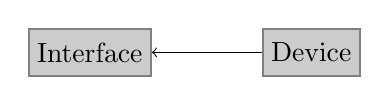
\begin{tikzpicture}[scale=1,inner sep=3pt, minimum size=6mm]
      \node [transition] (interface) {Interface};
      \node [transition] (device) [right of=interface, node distance=80pt] {Device};
      \draw [->] (device) -- (interface);
    \end{tikzpicture}\\
    优点:约束力强,静态约束\\
    缺点:考虑新增一个能力的情况,如果更新接口,那么所有设备都必须更新实现,否则无法通过编译,即使在中间引入一个默认实现类,那也只能处理一些有固定算法的情况,例如线绘制之类,一些如图形编码问题则只有依赖宏实现。\\
    \\
    方案二:\\
    \\
    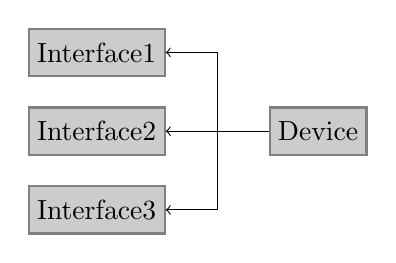
\begin{tikzpicture}[auto, scale=1,inner sep=3pt, minimum size=6mm]
      \node [transition] (interface1) {Interface1};
      \node [transition] (interface2) [below of=interface1] {Interface2};
      \node [transition] (interface3) [below of=interface2] {Interface3};
      \node [transition] (device) [right of=interface2, node distance=80pt] {Device};
      \draw [<-] (interface2.east) -- node[name=u]{}(device.west);
      \draw [<-] (interface1.east) -| (u.south);
      \draw [<-] (interface3.east) -| (u);
    \end{tikzpicture}\\
    新增一个能力时,可以直接新建一个接口。在使用时,查询设备是否支持,如果不支持就使用兼容实现\\
    优点:约束能力强,灵活\\
    缺点:对于没有元信息的c/c++,实现复杂\\
         使用复杂(虽然是在系统内部,但是这会造成大量重复的判断代码,违背TRY原则)。\\
    \\
    方案三:\\
    \\
    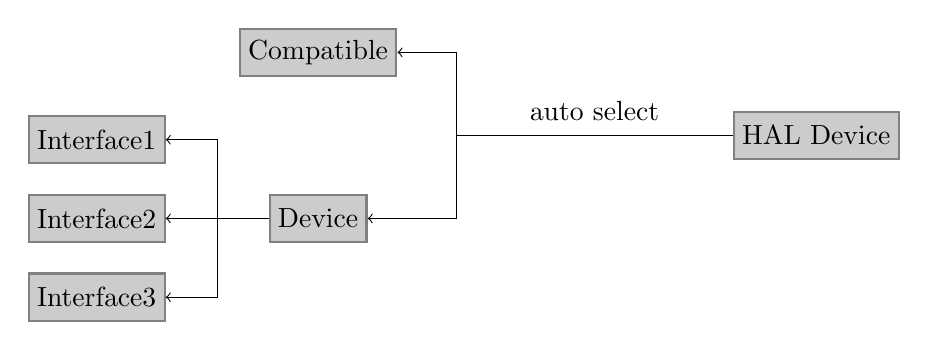
\begin{tikzpicture}[auto, scale=1,inner sep=3pt, minimum size=6mm]
      \node [transition] (interface1) {Interface1};
      \node [transition] (interface2) [below of=interface1] {Interface2};
      \node [transition] (interface3) [below of=interface2] {Interface3};
      \node [transition] (device) [right of=interface2, node distance=80pt] {Device};
      \draw [<-] (interface2.east) -- node[name=u]{}(device.west);
      \draw [<-] (interface1.east) -| (u.south);
      \draw [<-] (interface3.east) -| (u);
      
      \node [transition] (compatible) [above of=device, node distance=60pt] {Compatible};
      \node (space) [above of=device, node distance=30pt] {};
      \node [transition] (haldevice) [right of=space, node distance=180pt] {HAL Device};
      \node (y) [right of=space, node distance=50pt] {};
      \draw (y.center) -- node {auto select} (haldevice);
      \draw [<-] (compatible.east) -| (y.center);
      \draw [<-] (device.east) -| (y.center);
    \end{tikzpicture}\\
    auto select 通过查询能力,来选择,如果设备不支持就使用内置实现。\\
    这个可以看成是方案二的二次包装。\\
    \\
    ACGE选择: 方案三\\
    \\
    具体实现:\\
    Interface采用COM的基础结构。保留Query通过char*查询以保留外部拓展性。\\
    \\
    通过引入状态机,减少参数传递。\\

\section*{2014.11.23}
色彩机制:\\
不同设备对色彩支持不一致,具体表现为:\\
1.格式不同,浮点,整型\\
2.编码不同,AARRGGBB,RRGGBB,RGB,ARGB,BBGGRRAA等\\
同时HAL需要支持多种色彩形式。\\
\\
device编写者处理浮点精度问题和转换问题。\\
\\
IRGBColor, IRGBFColor, IARGBColor, IARGBFColor\\
\\
开始实现framebuffer device\\

\section*{2014.11.26}
修改接口机制\\
增加ClearSuffer图形设备接口\\

\section*{2014.12.2}
开始实现gdiplus device\\

\section*{2014.12.12}
修改接口约定,一个设备的实现类,必须使用一个void createInstance()来导出。\\
修改GraphicsDevice接口,增加初始化图形环境的要求。\\
增加平台工具类dynamic linker,来支持跨平台的动态加载链接库\\
增加图形设备工程\\
引入json解析库 -- rapidjson\\

\section*{2014.12.16}
引入GraphicsContext,其实例只保证本次调用内的生命周期。\\
GraphicsContext在不同的系统下有不同的定义,是保证多平台的基础。\\

\end{document}